
It has been shown that the number of charged particles with transverse
momentum (\pT ) above 500\,MeV, \ntrk, associated with a jet can be used
to select samples which have an increased fraction of jets produced by
quarks (or gluons). Samples with enhanced fractions of quark or gluon
initiated jets can be created by using a selection based on the \ntrk\
as shown in Fig.~\ref{fig:jet_pt_quark_gluon}.
Ref.~\cite{ATL-PHYS-PUB-2017-009} also shows that the \Pythia8
generator~\cite{pythia8} using the A14 tune~\cite{A14tune} is in a good
agreement with the distributions found in data.


\begin{figure}[htb]
 \centering
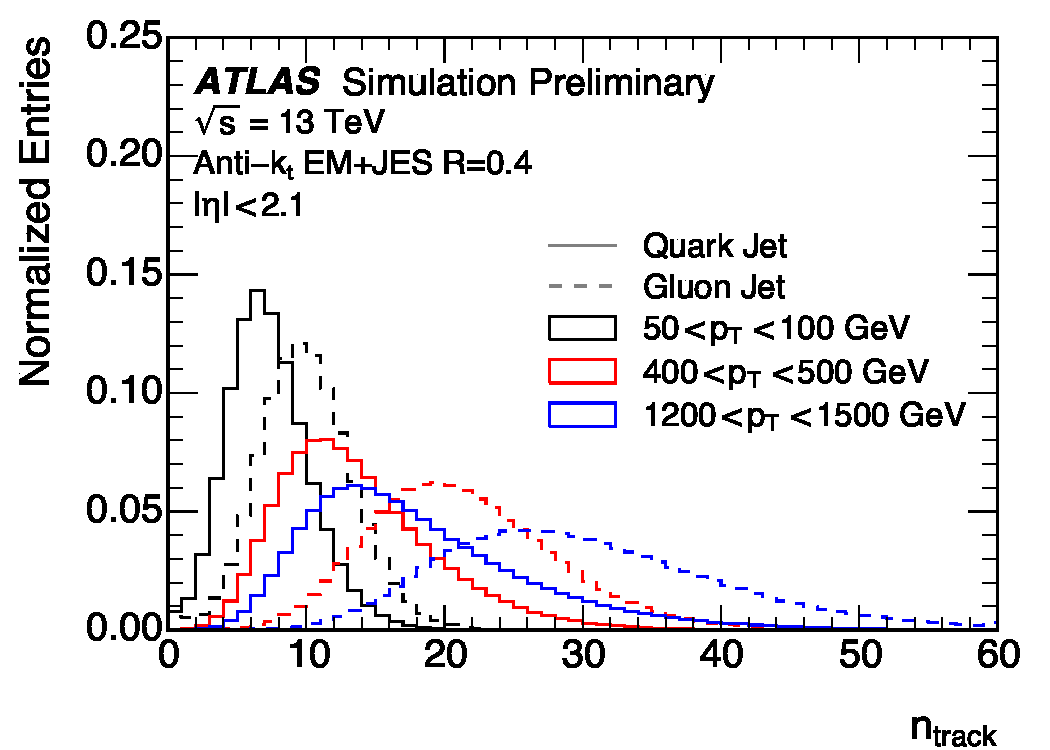
\includegraphics[width=0.75\textwidth]{figures/tagging/fig_01_ATL-PHYS-PUB-2017-009.pdf}
\caption{Distribution of the jet reconstructed track multiplicity (\ntrk ) in
 different pT ranges with the \Pythia~8 generator~\cite{pythia8} using
 the A14 tune~\cite{A14tune}, the NNPDF2.3 PDF
 set~\cite{Carrazza:2013axa}, and processes with a full simulation of the
 ATLAS detector. Jets must be fully within the tracking acceptance
 ($|\eta|<2.1$) and tracks are required to have $\pT > 500$\,MeV and pass
  quality criteria described in Ref.~\cite{ATL-PHYS-PUB-2017-009}. Figure
 from Ref.~\cite{ATL-PHYS-PUB-2017-009}. \label{fig:jet_pt_quark_gluon}}
\end{figure}

In Ref.~\cite{ATL-PHYS-PUB-2017-009}  the selection criteria for  an enriched quark-initiated jet sample was chosen so that 
each \pT\ bin had 60\% quark-initiated purity. Applying this criteria to the high mass dijet sample would lead to 
discontinuities in the mass spectrum that would present difficulties to a resonance search. Two alternative selection
criteria have been investigated, one based on that used in Ref.~\cite{ATL-PHYS-PUB-2017-009} and a simple linear
alternative. A jet is classed as being quark-initiated if \ntrk is less than the threshold \nqg\ (Eq.~\ref{eq:QGselect}):

\begin{align}
\ntrk & < \nqg \; \mbox{quark-initiated sample} \label{eq:QGselect} \\
	  & \ge \nqg \; \mbox{gluon-initiated sample} \nonumber
\end{align}

The implementation of the selection criteria used in Ref.~\cite{ATL-PHYS-PUB-2017-009} used here sets \nqg\ to 
\begin{equation}
\nqg = \mathrm{int} \left[ \frac{65}{1 + \exp\left[-0.003 (\pT - 1500) \right]} +7 \right]  \label{eq:nqg1} 
\end{equation}
where the \pT\ is measured in GeV and int truncates the value to an integer. The alternative selection criteria uses a linear function of the \pT
\begin{equation}
\nqg = {m \ln(\pT) + c}  \label{eq:nqg2}
\end{equation}
where m and c are constants chosen to provide suitable subsamples.
These selection criteria are applied to the two leading jets to separate dijet events into three samples:
where both jets are more likely to be quark-initiated, \QQ,  where both jets are more likely to
be gluon-initiated, \GG, and where we have one of each, \QG.
Simulated background events are separated into sub-samples based on the selection criteria given in
Eqs.~\ref{eq:nqg1} and \ref{eq:nqg2} and are shown in Fig.~\ref{fig:pythia_qg_selection}. It is clear that
the selection using Eq.~\ref{eq:nqg1} (Fig.~\ref{fig:pythia_qg_selection} a) produces more complex background shapes
than those Eq.~\ref{eq:nqg2} (Fig.~\ref{fig:pythia_qg_selection} b). Since the selection using  Eq.~\ref{eq:nqg2} will
be much easier to fit it will be used for initial toy-MC studies of limit setting. Alternative selections using Eq.~\ref{eq:nqg2} are produced for comparison, "selection 1" with m = 0.02, c = 0, and "selection 4" with m = 0.01, c = 15.


\begin{figure}[htb]
 \centering
  \subfigure[] {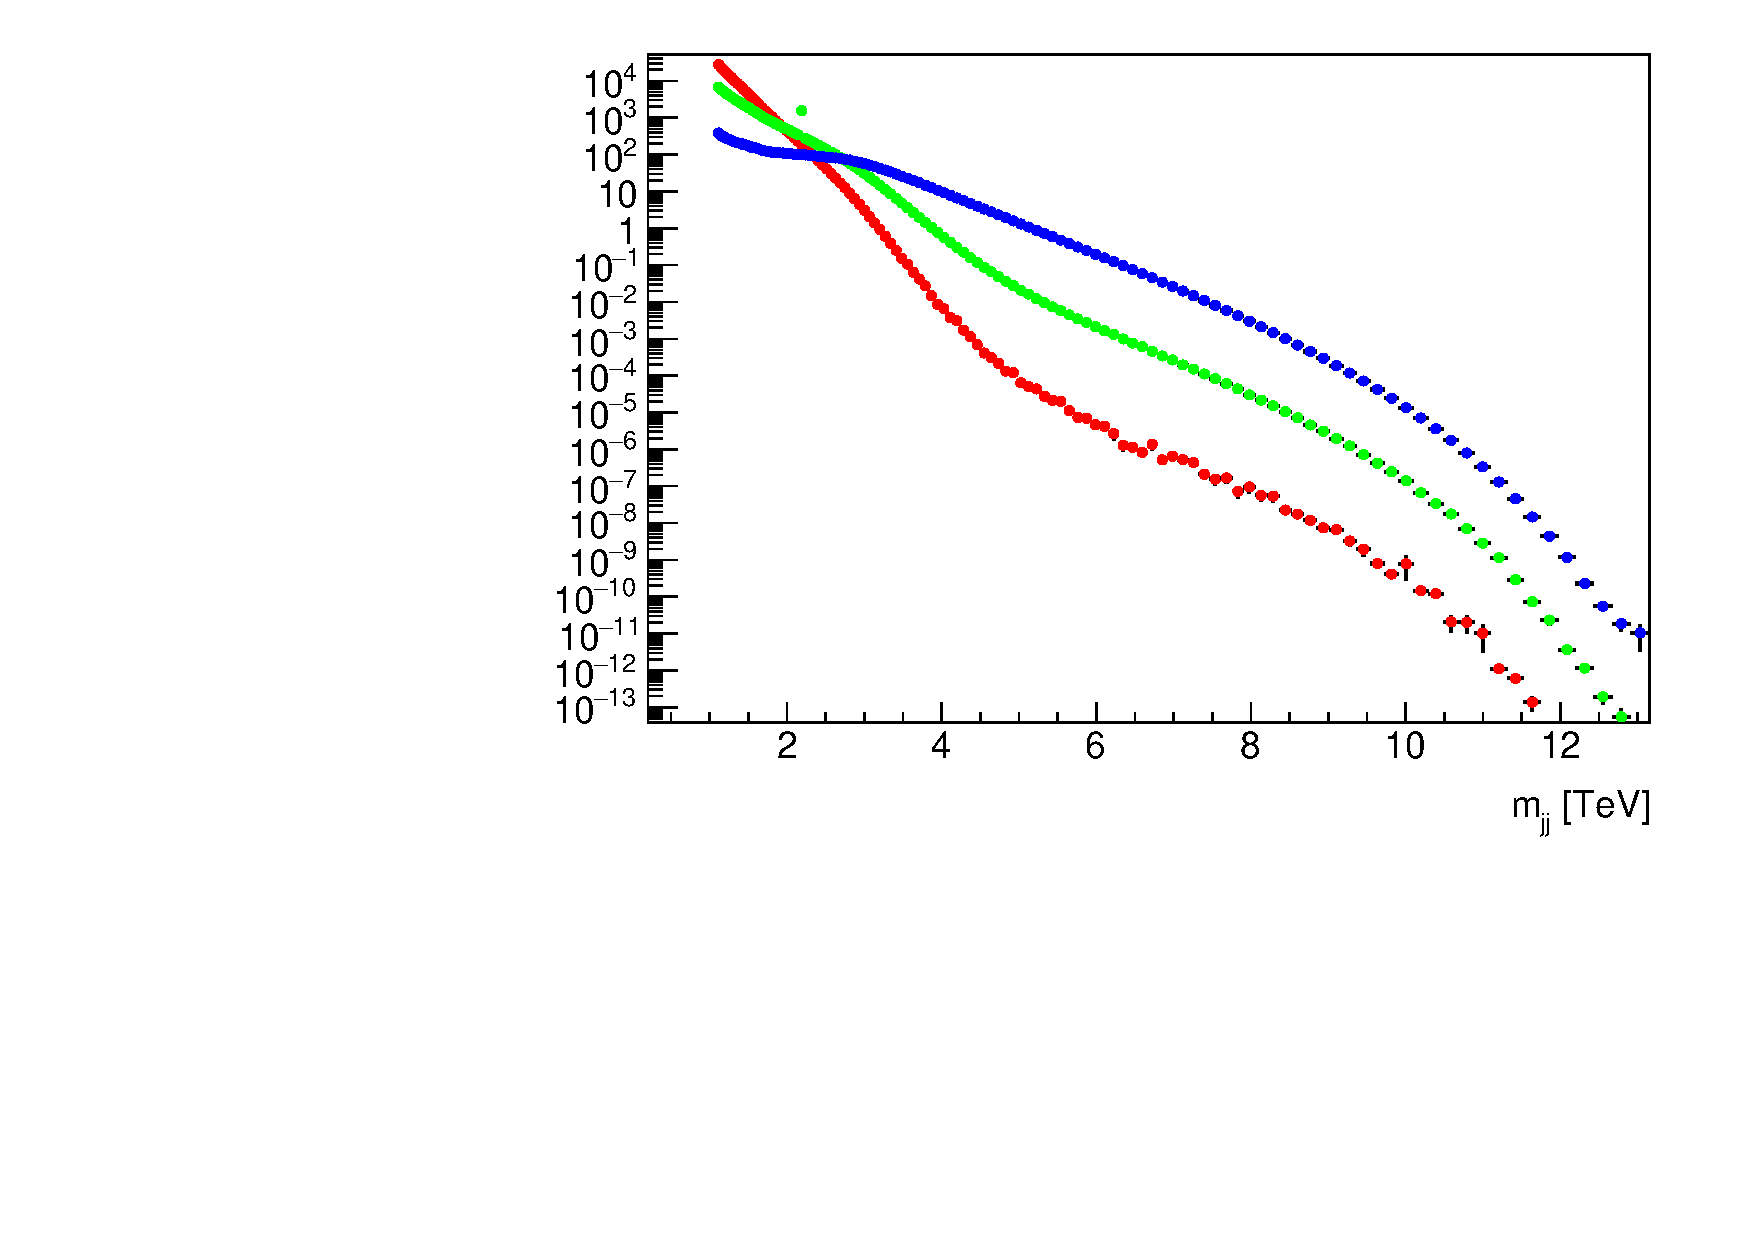
\includegraphics[width=0.495\textwidth]{figures/tagging/BackgroundQG_1.pdf}}
  \subfigure[] {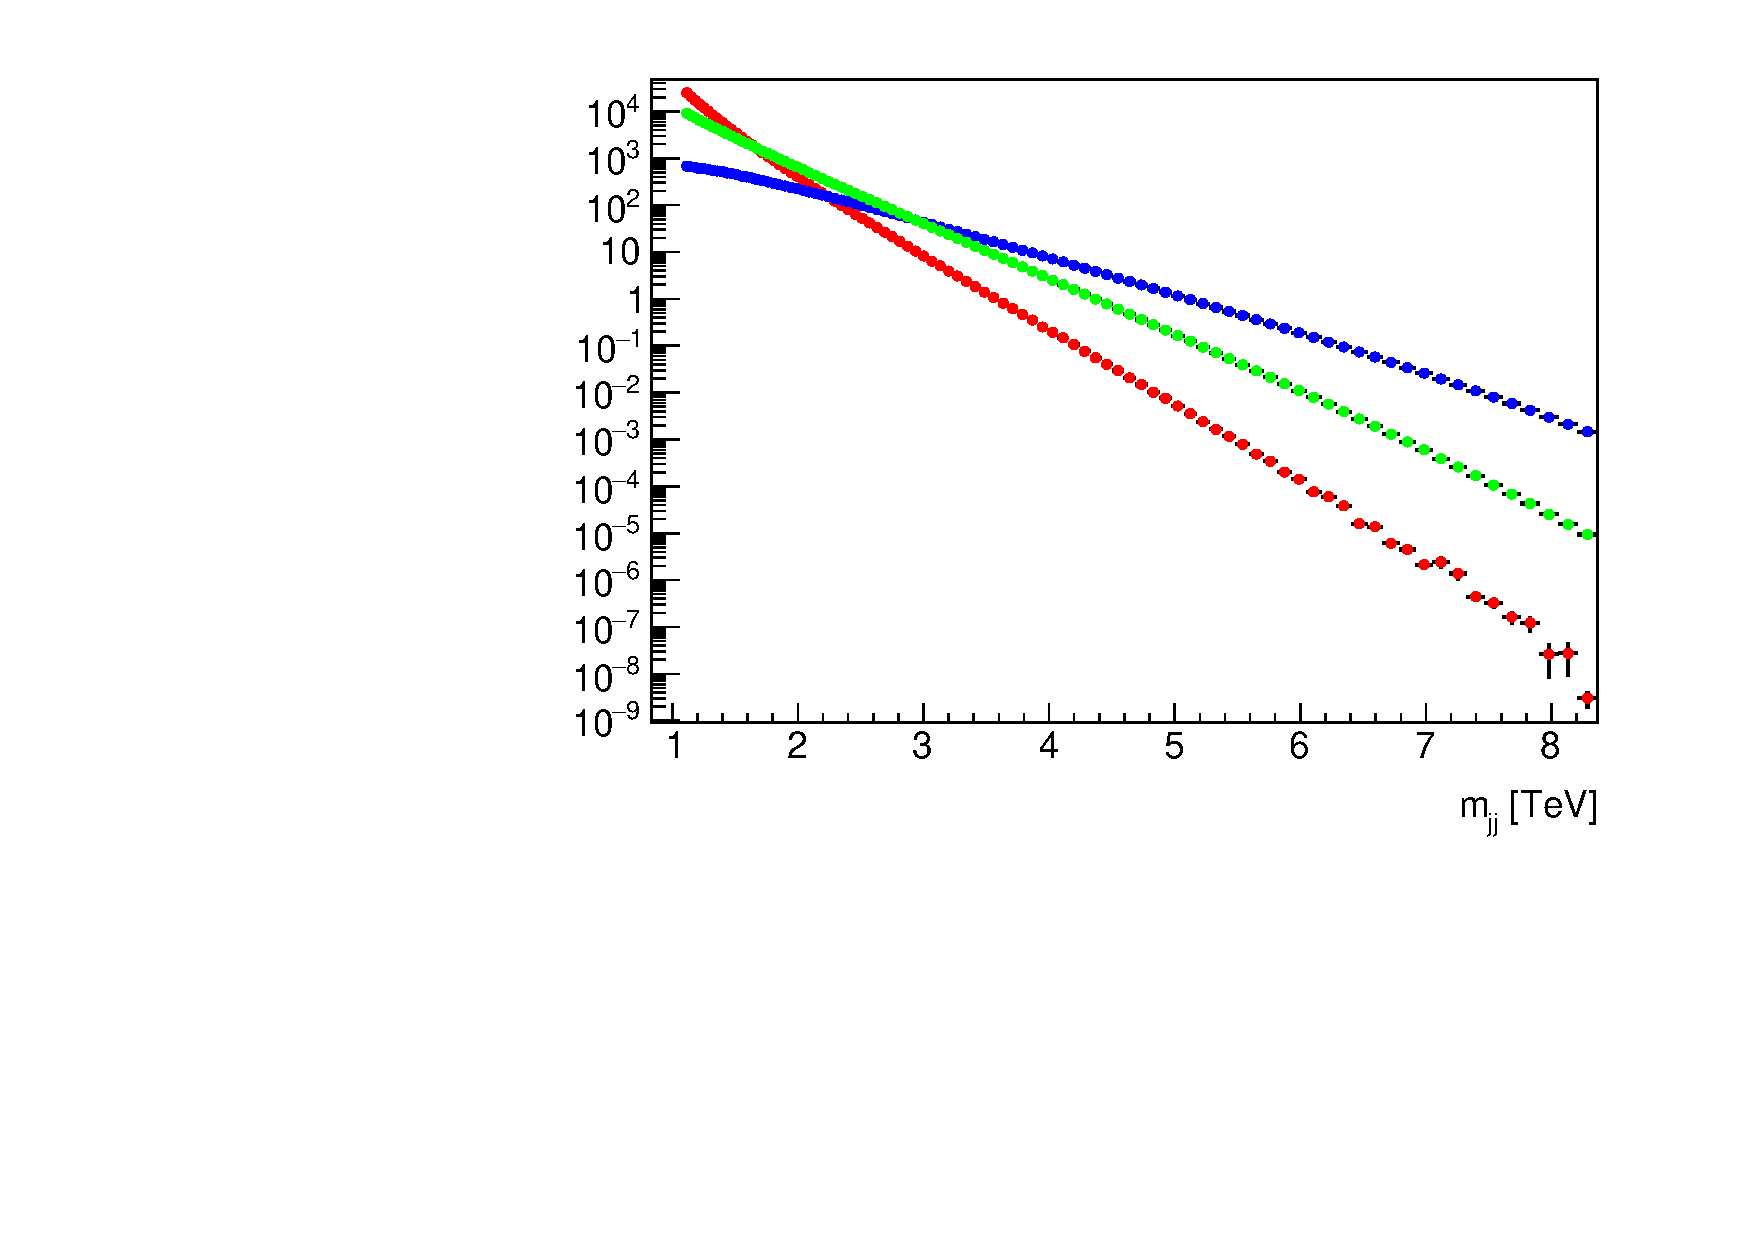
\includegraphics[width=0.495\textwidth]{figures/tagging/QG_linear.pdf}}

\caption{Simulated dijet samples produced using the 
\Pythia~8 generator~\cite{pythia8} using the A14 tune~\cite{A14tune}, the NNPDF2.3 PDF set~\cite{Carrazza:2013axa}, 
and processes with a full simulation of the ATLAS detector. The simulated events are separated into \QQ\ (blue),
\QG\ (green) and \GG\ (red) samples  based on (a) Eq.~\ref{eq:nqg1} and
(b) Eq.~\ref{eq:nqg2}.  \label{fig:pythia_qg_selection}}
\end{figure}

Figure~\ref{fig:QG_qstar_4tev} shows the selection applied to the mass distribution of a 4\,TeV \qstar . The  
\QQ sample is more peaked and has a smaller tail than the \QG\ distribution which has a similar shape to the complete signal. The \GG\ sample of high multiplicity jets has a very small peak and is dominated by the tail.

\begin{figure}[htb]
 \centering
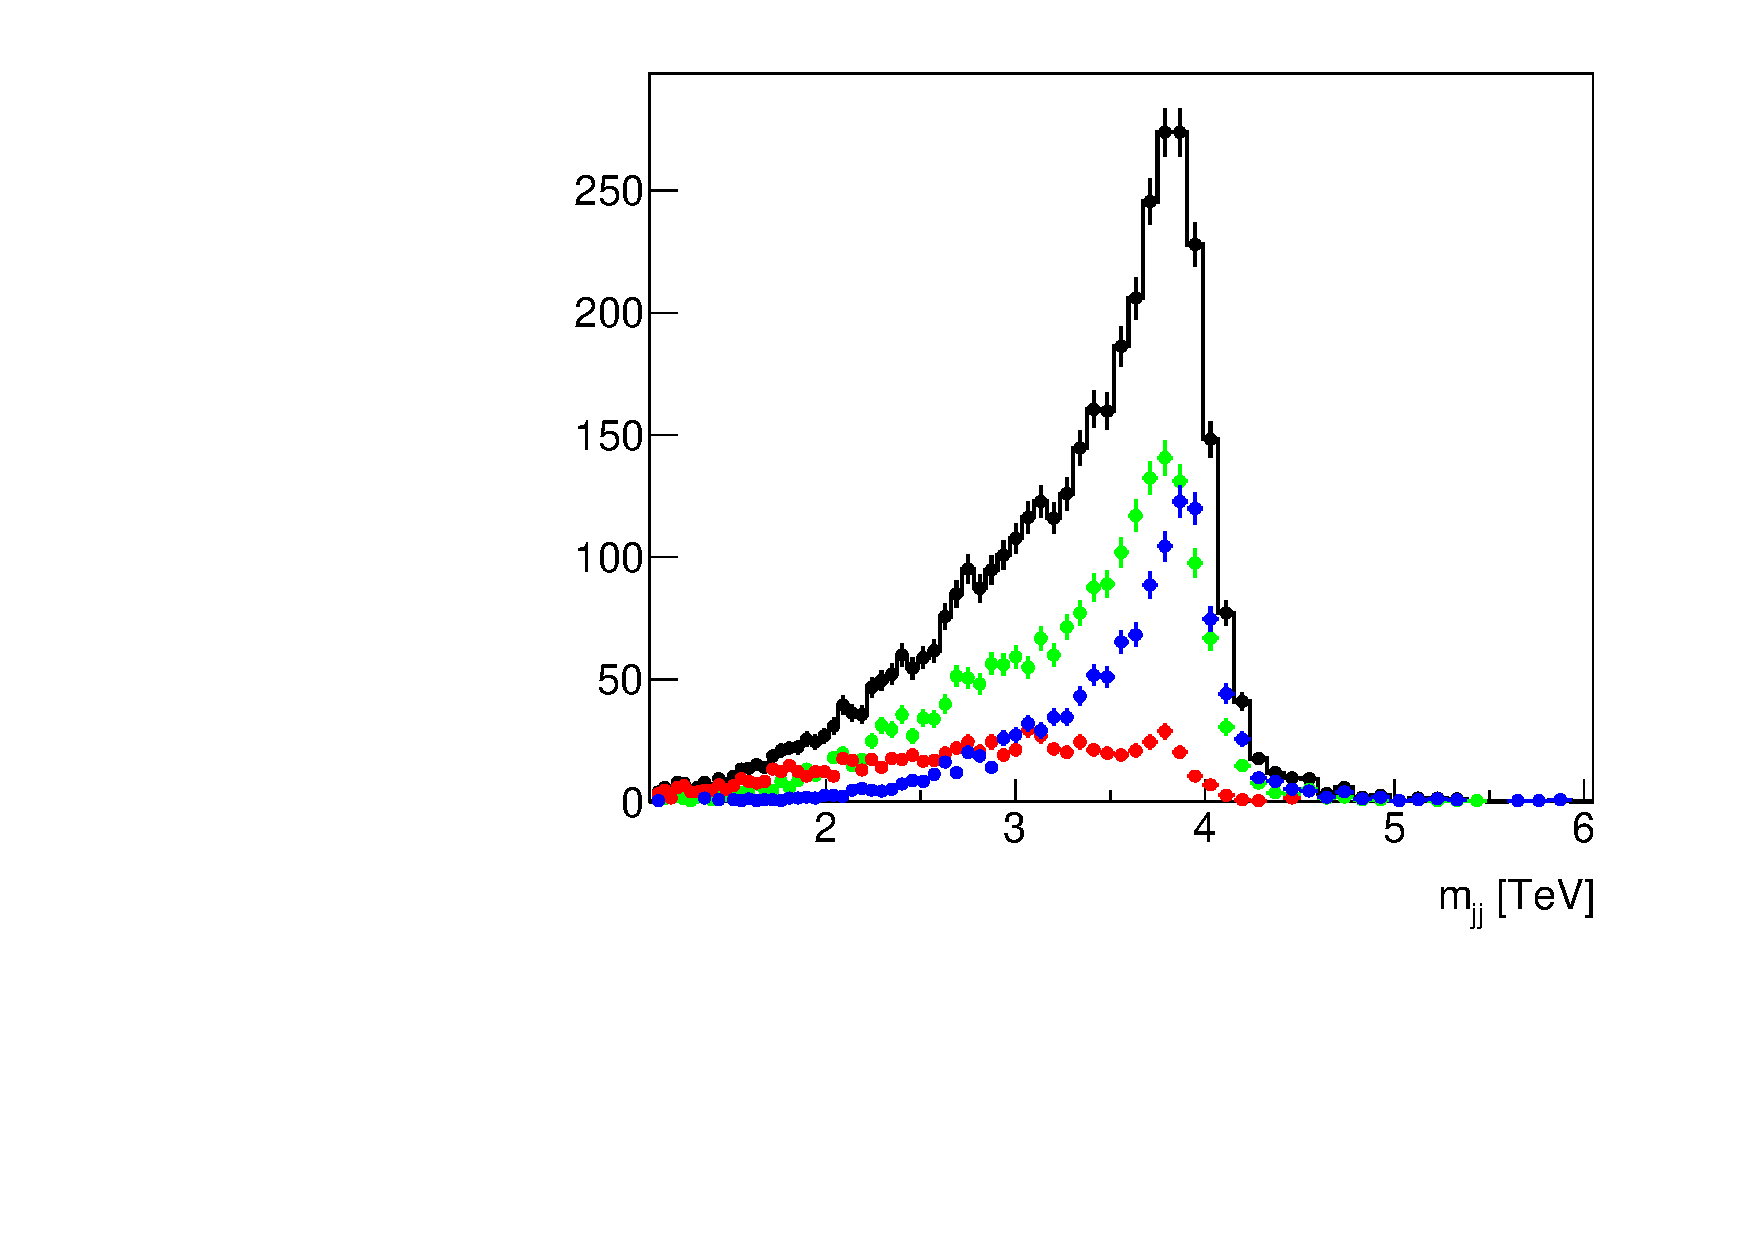
\includegraphics[width=0.75\textwidth]{figures/tagging/QG_qstar_4tev.pdf}
\caption{Simulated 4\,TeV \qstar\ sample seperated into \QQ\ (blue) , \QG\ (green) and \GG\ (red) 
sub-samples.  \label{fig:QG_qstar_4tev}}
\end{figure}

\clearpage
\subsection{Signal Fractions Quark-Gluon selection}

The fraction of \qstar\ signal events is measured for masses from 1\,TeV to 7.0\,TeV and are given in Table~\ref{table:qstar_fractions}. The low fraction of \QQ\ events at masses from 1 to 3\,TeV suggest that
further optimisation of the selection criteria are required.  

\begin{table}[h]
	\centering 
		\caption{The fraction of \qstar\ MC events in the \QQ, \QG, and \GG\ sub-samples for various masses. 
		\label{table:qstar_fractions}}
	\begin{tabular}{SSSS}
	\toprule
\qstar\ Mass (TeV) & \multicolumn{1}{c}{\QQ\ Fraction} &  \multicolumn{1}{c}{\QG\ Fraction}  &  \multicolumn{1}{c}{\GG\ Fraction} \\
\midrule 
1.0	&	0.06 &	0.31 &	0.63\\
2.0	&	0.04 &	0.37 &	0.59\\
2.5	&	0.09 &	0.45 & 	0.46\\
3.0	&	0.15 &	0.51 &	0.35\\
3.5	&	0.22 &	0.53 &	0.25\\
4.0	&	0.30 &	0.51 &	0.19\\
4.5	&	0.37 &	0.48 &	0.15\\
5.0	&	0.44 &	0.44 &	0.12\\
5.5	&	0.49 &	0.41 &	0.10\\
6.0	&	0.53 &	0.37 &	0.09\\
6.5	&	0.56 &	0.35 &	0.09\\
7.0	&	0.57 &	0.33 &	0.10\\
\bottomrule
\end{tabular}
\end{table}


\begin{figure}[htb]
 \centering
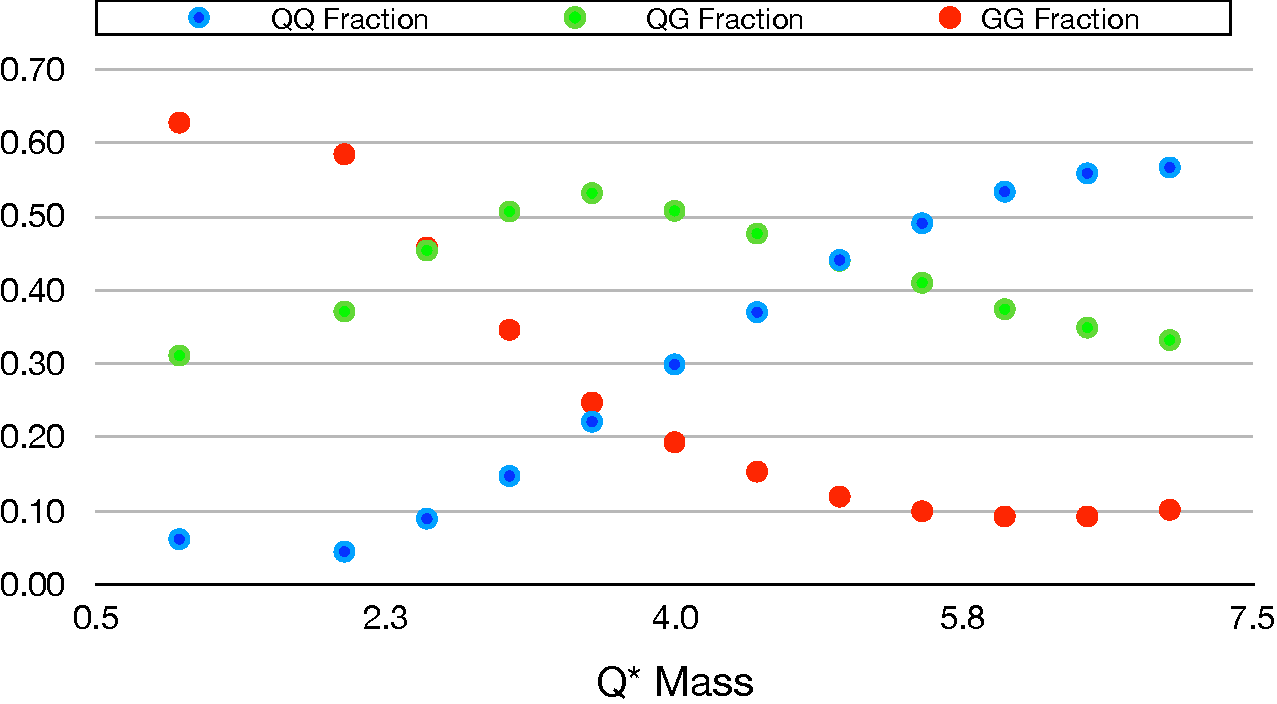
\includegraphics[width=0.75\textwidth]{figures/tagging/QStarEfficincies.pdf}
\caption{The fraction of \qstar\ MC events in the \QQ, \QG, and \GG\ sub-samples for various masses.   \label{fig:QStarEfficincies}}
\end{figure}



\subsection{Signal Morphing with Quark-Gluon selection}

Signal morphing (Sec.\ref{sec:SwiftMorphing}) is applied to the \qstar\ signal subsamples. The MC signal 
sub-samples for \QQ\ and \QG\ are fit to a Gaussian + reverse Landau function, a parameterization that has 
one normalization  and five shape parameters. The parameters are interpolated as a function of mass using cubic splines.
%\textit{ \color{red} The \GG\ subsamples have not been morphed at this time.} 

